\section{Speech Interface}
\label{sec:speech}

Voice is the primary interface; typing is a fallback. Speech recognition (STT) and synthesis (TTS) run in a separate local
service. TTS is used off the shelf. STT was first used off the shelf (\S\ref{sec:stt}--\ref{sec:noise}); the deployed
recognizer is a version fine-tuned on car commands (\S\ref{sec:sttft}).

\subsection{Recognition, numbers and end-to-end accuracy}
\label{sec:stt}

\paragraph{Setup.} Candidates were Parakeet-CTC-0.6B-Vietnamese \citep{nvidia2026parakeetvi} (exported to ONNX, int8),
PhoWhisper-small and PhoWhisper-medium \citep{le2024phowhisper} (CTranslate2 int8 via faster-whisper), all on 8 CPU threads
with greedy decoding. TTS is VieNeu-TTS \citep{vieneu2026tts} (0.1B, 48\,kHz, ONNX on CPU, female northern voice). The
recognizers write numbers as words (\textit{hai mươi hai độ}, ``twenty-two degrees''), whereas the student was trained on
digits, so transcripts go through a normalizer that converts spoken numbers to digits, removes final punctuation and
capitalizes the first letter. The end-to-end metric is: speech $\rightarrow$ STT $\rightarrow$ normalizer $\rightarrow$
deployed model $\rightarrow$ rule-C scoring against the frozen reference, alongside the same chain fed with the original
text (``typed''). Set A (230 clean-test sentences read by 25 synthetic voices) served only for debugging; sets B, C and D
(40, 30 and 30 sentences sampled from frozen test sets, each list locked before reading) were recorded by the first author with
a laptop microphone in a quiet room.

\begin{table}[t]
\centering\small
\setlength{\tabcolsep}{3.5pt}
\begin{tabular}{@{}lcccc@{}}
\toprule
Set B (40, real voice) & Correct & WER & p50 & p95 \\
\midrule
Typed (same chain) & 30 & -- & -- & -- \\
Parakeet-CTC 0.6B & 15 & 33.3 & 388\,ms & 489\,ms \\
PhoWhisper-small & \textbf{21} & 20.2 & 1,844\,ms & 4,716\,ms \\
PhoWhisper-medium & 18 & \textbf{17.0} & 4,806\,ms & 5,136\,ms \\
\bottomrule
\end{tabular}
\caption{STT selection (pre-registered rule: most end-to-end correct; within two items, lower p95 latency). Measured before
the number-normalization fix.}
\label{tab:stt}
\end{table}

\paragraph{Choosing the recognizer.} PhoWhisper-small won the pre-registered comparison (Table~\ref{tab:stt}).
PhoWhisper-medium had the lowest word error rate but fewer correct commands: WER weighs every word equally, while one wrong
number or part name breaks a command (medium heard ``25 degrees'' as \textit{hai găm độ}). Synthetic speech overrated
Parakeet (WER 21.5\% on set A, 33.3\% on real voice): the CTC model glues or splits syllables on real speech, while the
Whisper decoder uses linguistic context.

\paragraph{A bug found by real voice.} Of the 11 commands PhoWhisper-small lost on set B, three were caused by our own
normalizer: Vietnamese speakers say \textit{hai hai độ} for 22 degrees, and the normalizer added the digits (4 degrees). After
the fix, a new set C gained four commands (17 $\rightarrow$ 21 of 30), all colloquial numbers; set A, read by TTS voices that
pronounce numbers in full, did not change at all. Re-scoring set B after the fix (22 of 40) is reported only as post-hoc.
Vocabulary hints and beam search were then compared on a new set D under a pre-registered rule: greedy without hints scored
17, hints 16, beam 5 17, both 16, so greedy was kept.

\paragraph{End-to-end.} The headline numbers for the off-the-shelf recognizer pool the 60 new sentences of sets C and D:
\textbf{42 of 60 (70.0\%) typed and 38 of 60 (63.3\%) spoken}, so speech costs 6.7 points. Per set the drop was 22.5 points on B (before the
fix), 10 on C and 3.3 on D. For context, SFC-Bench reports drops of 17--20 points for 8B--32B models at its easiest level
\citep{peng2026sfc}; the settings differ in language, functions, metric and speech (synthetic there, one real speaker here),
so we place our numbers in that range rather than compare them. The remaining speech errors are real mishearings---n/l and
tr/ch confusions (\textit{Nội Bài} $\rightarrow$ \textit{lộ tài}), \textit{độ} (degree) $\rightarrow$ \textit{đội}---which the
model mostly handles by refusing or asking rather than acting.

\subsection{Noise robustness}
\label{sec:noise}

All recordings were made in a quiet room, and the system has no denoising stage. With the off-the-shelf recognizer, we mixed the 60 C+D recordings with three
noises at 20, 10, 5 and 0\,dB SNR relative to the speech portion: real in-car noise (DEMAND \code{TCAR}, \citealp{thiemann2013demand}),
synthetic brown noise and Vietnamese background speech from FLEURS \citep{conneau2023fleurs}. The pre-registered rule was to try a
denoiser only if in-car noise at 10\,dB cost more than 6 of 60 commands.

\begin{figure}[t]
\centering
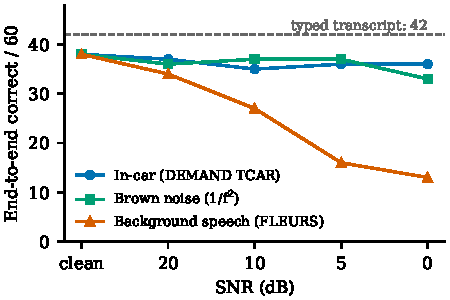
\includegraphics[width=\columnwidth]{figures/noise.pdf}
\caption{End-to-end correct commands (of 60) under additive noise.}
\label{fig:noise}
\end{figure}

In-car noise at 10\,dB cost 3 commands, so no denoiser was added (Figure~\ref{fig:noise}). PhoWhisper's WER stayed at about 22\% for
in-car noise down to 0\,dB; differences of one to three commands are within noise for 60 items. The real weakness is
\emph{another person speaking}: at 10\,dB the chain lost 11 commands, and at 5\,dB the recognizer transcribed the background
speaker as well (WER above 100\%), leaving 1 of 35 clear commands. The failure is safe: out-of-scope items stayed at 10--11 of
12, because the model refuses garbled text instead of acting on it. Single-channel denoisers target stationary noise and cannot
separate a second voice; multi-microphone hardware or source separation would be needed. Music was not tested. Separately,
browser audio processing (noise suppression and automatic gain) removed high-frequency consonants in the demo
(\vi{nóng quá}{so hot} heard as \textit{lóng quá}); requesting raw audio made the demo match the measured condition.

\subsection{Improving recognition}
\label{sec:sttft}

In live use the recognizer felt worse than the measured 63\%, so we looked for the cause and for a remedy, reusing the
recordings. Every remedy was selected on set B and checked on other data under a rule written down beforehand; sets C and D
were reused three times in this subsection and are therefore not used for the final numbers.

\paragraph{The demo's audio path is not the cause.} We replayed the 60 C+D recordings through the real interface: Chromium
used each file as a fake microphone, the page recorded it with \code{MediaRecorder} (WebM/Opus) and posted it to the same
service. The chain was correct on 36 of 60 commands, against 38 when the WAV files were sent directly (exact McNemar
$p=0.63$); half of the transcripts differed, but in both directions. The recognizer itself is the bottleneck: it misrecognizes
22\% of the words even on the original files, and tiny changes in the audio change its output.

\paragraph{Three training-free remedies did not help.} (i) A different recognizer: Zipformer-30M
\citep{yao2023zipformer,hynt2025zipformervi}, a 30M-parameter transducer run with sherpa-onnx, was ten times faster (median
0.17\,s vs.\ 1.75\,s) and had a lower WER (15.7\% vs.\ 22.0\% on C+D), yet produced \emph{fewer} correct commands (20 vs.\ 22
on B; 32 vs.\ 38 on C+D, $p=0.18$). Its errors fall on the words that select a function---\textit{nắp xăng} (fuel flap)
$\rightarrow$ \textit{lắp sang}, \textit{cốp} (trunk) $\rightarrow$ \textit{cúp}---whereas PhoWhisper's fall on sentence-final
particles and filler words that the language model ignores. It failed the pre-registered rule (three more correct commands
on B); a rule relaxed after seeing set B (lower WER, not significantly worse) would have admitted it, but with fewer correct
commands on both sets we kept PhoWhisper. As with PhoWhisper-medium above, average WER is the wrong yardstick for spoken
commands. (ii) Running both recognizers and keeping the transcript on which the language model is more
confident gave exactly PhoWhisper's score (22 of 40; 38 of 60), although an oracle choice would reach 25 and 42: the
decision-token confidence tells whether a sentence is a clear command, not whether it was heard correctly, so the model is
just as confident on \textit{lắp sang}. (iii) Repairing misheard multi-syllable part names with the initial-consonant
confusions common across Vietnamese regions (l/n, s/x, ch/tr, d/gi/r), from a vocabulary written before any recording, changed
three PhoWhisper transcripts and no outcome (on 30,060 accented training sentences it altered 0.37\%, mostly injected
typos).

\paragraph{Fine-tuning the recognizer.} We then fine-tuned PhoWhisper-small on in-domain audio: 5,000 command sentences from
the language model's \emph{training} data (contamination-checked against all test sets and recording sets), with digits
spelled out and read by 23 of the 25 VieNeu voices; 1,500 FLEURS training utterances to preserve general Vietnamese; and, for
variant B only, 150 new sentences read by the first author (12 minutes, repeated four times). Each sample is degraded at
random while training: speed 0.9--1.1, synthetic reverberation, DEMAND in-car noise at 0--20\,dB SNR, a laptop-microphone
band-pass and gain. Training takes three epochs at learning rate $10^{-5}$ (6--8 minutes on an A100); each epoch is converted
to the same CTranslate2 int8 format, so latency is unchanged. The checkpoint was chosen on set B (ties by lower WER) and
evaluated once on a new 40-sentence set E recorded for this purpose; forgetting was checked on 300 FLEURS test utterances and on
set G, 60 frozen-test commands read by the two VieNeu voices held out from training.

\begin{table}[t]
\centering\small
\setlength{\tabcolsep}{3.2pt}
\begin{tabular}{@{}lcccc@{}}
\toprule
& Set B & \multicolumn{2}{c}{Set E (final)} & FLEURS \\
\cmidrule(lr){3-4}
Recognizer & /40 & /40 & WER & WER \\
\midrule
Typed (same chain) & 30 & 32 & -- & -- \\
PhoWhisper-small & 22 & 24 & 24.8 & 11.6 \\
\quad + TTS and FLEURS (A) & 23 & 25 & 21.2 & 10.7 \\
\quad + 12 min real voice (B) & \textbf{25} & \textbf{28} & \textbf{14.5} & 10.8 \\
\bottomrule
\end{tabular}
\caption{Fine-tuning the recognizer: end-to-end correct commands with the deployed language model, and word error rate
(\%). Set B selected the checkpoint; set E was used once.}
\label{tab:sttft}
\end{table}

Table~\ref{tab:sttft} shows that synthetic speech alone barely helps on a real voice (and raised wrong actions on set E from
6 to 9), while adding 12 minutes of real recordings cuts the word errors by 40\% and recovers half of the gap to typed input
(24 $\rightarrow$ 28 of 32), with wrong actions unchanged at 6. What the off-the-shelf recognizer lacked was therefore
acoustic---this voice and this microphone---rather than vocabulary. Variant B is deployed. Three cautions apply. The gain on
set E is five commands won and one lost ($p=0.22$), not significant with 40 items, though consistent with set B. Set E shares
its speaker, microphone and recording session with the fine-tuning recordings, so it measures the benefit for \emph{this}
speaker. And for other speakers we could only show absence of harm: FLEURS WER did not rise, and on set G correct commands
went from 29 to 46 of 60 for both variants---a figure inflated by the shared TTS engine, which we read only as ``no harm''. A
check on other real speakers giving commands is missing; the noise and wake-word experiments were run with the original
recognizer.

\subsection{Wake word}
\label{sec:wake}

``Hey Nexa'' lets the driver start a command hands-free. Porcupine's free tier is no longer available and running STT
continuously costs about 1.8\,s of CPU per utterance, so we trained a detector on openWakeWord's
\citep{scripka2023openwakeword} frozen feature extractors (mel spectrogram and a speech embedding model,
\citealp{lin2020kws}): 16 frames of 96 dimensions (1.28\,s) feed a small scikit-learn MLP, updated every 80\,ms. A detection
requires $k$ consecutive frames above a threshold, followed by a 2\,s refractory period; Silero VAD \citep{silero2024vad} ends the
command after silence, and the wake phrase is stripped from the transcript. Wake-word commands carry the source
\code{wake\_word}, which activates the confirmation rules of Table~\ref{tab:safety}; the detector pauses while the assistant
speaks.

Version 1 used only synthetic positives (VieNeu reading six Vietnamese spellings of ``hey nexa'' with 20 voices, 5 held out),
synthetic negatives (near-miss phrases, car commands, the assistant's own replies), Vietnamese FLEURS training audio and 500k
precomputed ACAV100M feature windows \citep{lee2021acav100m}. It caught 98.9\% of held-out synthetic calls but only 16 of 40 of
the first author's real calls. The recordings peaked at $-23$ to $-38$\,dBFS, whereas training positives peaked at $-18$ to $-3$\,dBFS, and fast calls rarely stayed
above threshold for the required four frames. Version 2 widened the level augmentation to $-46\ldots-3$\,dB, added 46 real
training calls (14 held out for validation, none from the test recordings), and re-selected $k$ and the threshold on
validation.

\begin{table}[t]
\centering\small
\setlength{\tabcolsep}{4pt}
\begin{tabular}{@{}lccc@{}}
\toprule
& v1 & v2 & Target \\
\midrule
Real calls detected (40, new set) & 16$^{a}$ & \textbf{39} & $\ge$36 \\
False alarms / h (FLEURS test, 3.15\,h) & \textbf{1.27} & 2.86 & $\le$1 \\
Triggers on 30 spoken car commands & -- & 1 & 0 \\
Self-wake on assistant replies (38) & 0 & 0 & 0 \\
\bottomrule
\end{tabular}
\caption{Wake-word test (each measured once). $^{a}$On the first recording set. Rules: v1 four frames $\ge0.05$; v2 three
frames $\ge0.85$. CPU: about 3.5\% of one core.}
\label{tab:wake}
\end{table}

Version 2 detects almost every real call in every style (normal, fast, quiet, from 1--1.5\,m, with \textit{ơi}, followed
directly by a command), but false alarms doubled on continuous read speech, and one of the author's car commands triggered it
(Table~\ref{tab:wake}). We deploy version 2 and report that it meets the detection target but not the false-alarm target. A false
wake-up either times out after about four seconds of silence or sends the next overheard sentence to the assistant, which
usually refuses it; sensitive functions always require confirmation for wake-word commands. Because ACAV100M features are
licensed CC BY-NC-SA, the detector may only be used non-commercially.

\subsection{Latency}
\label{sec:latency}

On the laptop CPU a spoken command takes about 2.5\,s from end of speech to the start of the spoken answer: STT about 1.8\,s
for a 2--5\,s utterance, the model about 0.5\,s, and TTS about 0.25\,s until the first audio. The answer is synthesized and
streamed chunk by chunk, and the interface plays each chunk while the next one is generated. On ten answers this cut the time
to first audio from a median of 798\,ms (worst 2.8\,s for a three-part answer) when waiting for the whole sentence to 241\,ms
(worst 285\,ms). Synthesis runs faster than playback (0.85\,s for 2.7\,s of audio), so chunks play without gaps. Each extra
segment of a multi-command utterance adds about 0.5\,s. The laptop's 4\,GB GPU is not used.
